%cahier des charges projet SR .

\documentclass[french,11pt,a4]{article}
\usepackage[french]{babel}
\usepackage{amsfonts}
\usepackage{graphicx}
\usepackage[utf8]{inputenc}
\usepackage[top=3cm,right=3cm,left=2cm,bottom=3cm]{geometry}

\usepackage{fancyhdr}
\lhead{E.S.I.L département informatique}
\rhead{Projet Système Répartis}
\chead{}
%\lfoot{Année universitaire 2008-2009}
\pagestyle{fancy}

\makeatletter
\def\maketitle{%
  \thispagestyle{empty}
  %\begin{center}\leavevmode

  \vfill
  \begin{flushright}
  
\includegraphics[width=4cm]{esil.jpg}
  \end{flushright}
  \par
  \normalfont
  \hrule height 2pt
  \par
  \begin{center}
    \huge \strut \@title \par
  \end{center}
  \hrule height 2pt
  \par
  \vskip 1cm
  	\vfill
         {\Large \@author\par}%
         \vskip 3.5cm
		\begin{center}
                {\Large Date : \@date\par}%
                \end{center}
                \null
                \cleardoublepage
}
\makeatother
  
\title{Internet Distributed Chat, un Chat décentralisé.\\
	\Large Cahier des charges
}
\author{
\begin{tabular}{|ll|}
\hline
Auteurs :
	& \normalsize{Guillaume Coré, Badiss Djafar, Axel Jacquet, Yoann Rocagel, Simon Wirth}\\
	& \small{Promotion 2010 du département informatique de l'ESIL.}\\
\hline
Tuteurs :
	& \normalsize{Traian Muntean et Nicolas Baudru.}\\
\hline
\end{tabular}
}

\begin{document}
\maketitle

\tableofcontents


%\addcontentsline{toc}{section}{Présentation du document}
%\addcontentsline{toc}{section}{Environnement de développement}
%\addcontentsline{toc}{section}{Présentation du projet}
%\addcontentsline{toc}{section}{Présentation du document}
%\addcontentsline{toc}{section}{Délais et livrables}

\newpage 






\section{Objet}

Le projet consiste à construire une application de discussion entre
différents pairs, de manière répartie. En effet, des systèmes comme IRC
existent déjà mais fonctionnent selon le schéma usuel
client/serveur. Ainsi, de telles applications sont vulnérables aux pannes
du serveur. Dans le cadre d'un système réparti chaque pair est à la
fois client et serveur. Éviter la centralisation du service permet de former un réseau plus robuste et moins sujet au contrôle ou à la répression sans nécessiter le déploiement d'une infrastructure matérielle spéciale.\\

Ce projet garde une certaine ligne de conduite quant à la sécurité. Tous les pairs seront mis en relation de manière indirecte mais il leur sera possible de créer à la demande des connexions sécurisées avec un ou plusieurs pairs sciemment choisis.\\

\section{Contexte}

Ce projet s’inscrit dans le cadre des modules de système d'exploitation et de système répartis, de
deuxième année d’école d’ingénieurs à l’ESIL. Ce projet sera réalisé par une équipe, composée de cinq personnes.
Cela nous permettra de nous placer en situation réelle dans la mesure où nous sommes maîtres d’oeuvres
par rapport à un client qui attend des résultats. Nous pourrons ainsi mettre en application nos connaissances
et acquérir de nouvelles compétences.
Le projet est supervisé par M. Muntean et M. Baudru.

\section{Contraintes}
\subsection{Environnement de développement}

Le projet sera entièrement implémenté en langage Java et sous GNU/Linux. La machine virtuelle employée sera celle de Sun et la librairie utilisée sera openJDK (1.6). Pour ce qui est des parties réseaux, l'utilisation des RMI (Remote Method Invocation) sera préférée aux simples sockets pour une meilleure illustration du cours de systèmes répartis. Le choix de Java pour la réalisation du projet peut s'expliquer par les facilités d'implémentation des processus concurrents que ce langage de programmation permet (notamment l'utilisation des ``threads'').\\

La coordination entre développeur se fait par le biais d'un gestionnaire de version, dans notre cas il s'agît de GIT.\\

Le projet est développé sous certaines hypothèses facilitant l'implémentation dans un premier temps :\\
\begin{itemize}
\item{Nous nous plaçons dans le cas des réseaux LAN.}
\item{Toutes les machines du LAN possèdent une version de Java et des
  RMI à jour (i.e : version > 5 et bonne configuration de RMId et
  RMIregistery).}
\end{itemize}

\subsection{Délais et livrables}

La prise de connaissance des sujets a été effectuée en février. Le présent cahier des charges est à rendre pour la fin du mois de mars. Une réunion est prévue pour le mois d'avril.

Le projet quant à lui doit être rendu pour le Jeudi 7 mai 2009, jour de la soutenance. Les livrables sont les suivants :

\begin{itemize}
\item{Le présent cahier des charges.}
\item{Une archive contenant l'ensemble des codes sources produits.}
\item{Une présentation devant le jury constitué de Trayan Muntean et Nicolas Baudru.}
\end{itemize}
Les documents destinés à un usage interne au groupe sont rédigés mais ne font pas l'objet d'une évaluation.
Un chat distribué

\section{Description fonctionnelle}
Lors du premier lancement de l'application, l'utilisateur n'est connecté à personne. Lorsqu'il ouvre le programme, il a la possibilité de gérer ses connexions directes : ce sont les pairs à qui il est connectés directement, eux même connectés à d'autres pairs, etc.\\

Une fonction \textbf{recherche} de pairs affiche les pairs disponibles sur le réseau local. Cela lui permet d'en choisir pour s'y connecter et d'ainsi se bootstraper sur le réseau et d'avoir ses premières connexions. Il peut également \textbf{ajouter} un pair spécifique en précisant son adresse IP.\\

Une fois connecté à des pairs, l'utilisateur peut discuter avec tous les autres utilisateurs du réseau, même ceux à qui il n'est pas directement connecté. Pendant l'utilisation il conserve la possibilité d'ajouter une connexion directe avec un autre pair du réseau en le sélectionnant dans la liste globale des utilisateurs.\\

Initialement, tout le monde peut discuter avec tout le monde dans le salon global. Cependant l'utilisateur peut demander à un ou plusieurs pairs du réseau une conversation privée. Une invitation au dialogue privé est envoyée à ces pairs et s'ils l'acceptent, la connexion \textbf{chiffrée} est établie.\\

\subsection{IHM}

\subsubsection{Swing}
\paragraph{}
Swing est une bibliothèque graphique pour le langage de programmation
Java, faisant partie du package Java Foundation Classes (JFC), inclus
dans J2SE.Nous avons choisi d'utiliser cette bibliothèque pour
plusieurs raisons :
\begin{enumerate}
\item{Swing offre la possibilité de créer des interfaces graphiques identiques quel que soit le système d'exploitation.}
\item{Cette bibliothèque est relativement simple d'utilisation.}
\item{Les composants de Swing ne requièrent pas d'allocation de ressources natives.}
\item{Nous avons déjà une expérience dans l'utilisation de cette bibliothèque graphique.}
\end{enumerate}

Nous allons maintenant voir en détail les fonctionnalités de notre IHM.

La fenêtre principale est composée de différentes zones qui ont chacune leur utilité. Sur le screenshot suivant nous pouvons voir une ébauche de l'aspect de cette fenêtre que nous allons décrire.
\begin{center}
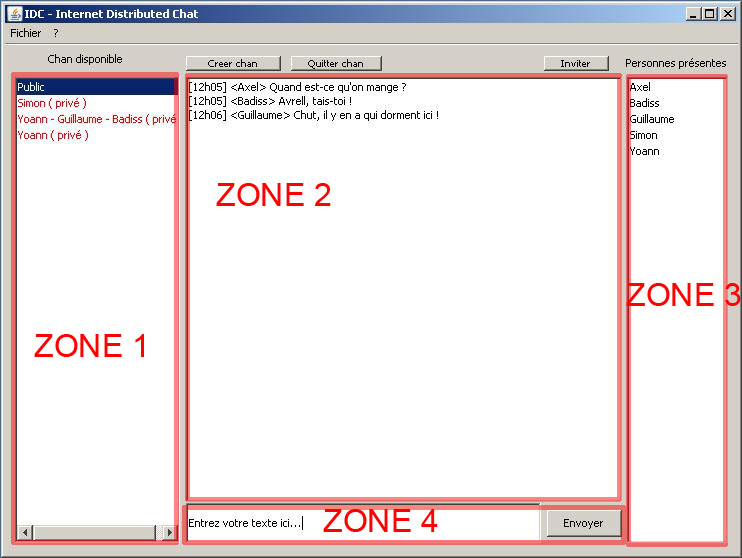
\includegraphics[width=15cm]{ImageSR1.jpg}
\end{center}
 
\begin{itemize}
\item{La zone 1 de la fenêtre permettra de voir les différentes
  personnes ou groupes de personnes avec lesquels nous pouvons
  discuter. Le simple fait de cliquer sur un de ces groupes permet
  d'afficher dans la zone 2 les discussions relatives a ce groupe et
  donne la possibilité d'écrire des messages qui seront transmis à
  toutes les personnes connectées à ce salon.}
\item{La zone 2 vous l'aurez compris permet d'afficher les conversations avec pour chaque commentaire l'heure d'envoi du message et le nom de l'émetteur.}

\item{La zone 3 permet de voir toutes les personnes connectées au réseau. Cette zone permet également d'inviter une personne à rejoindre un salon de discussion à l'aide du bouton 'inviter'.}

\item{La zone 4 servira à l'utilisateur pour pouvoir taper son message à envoyer sur le salon. Le bouton 'créer chan' ouvre une fenêtre qui demandera le nom du salon et de cocher les différentes personnes que le créateur souhaite avoir dans son salon. Le bouton 'quitter' déconnecte l'utilisateur du salon.}

\item{Dans le menu fichier l'onglet 'Gérer les connexions' affichera une fenêtre qui donnera des informations sur les pairs directs (nom, adresse IP, id). Cette fenêtre permettra également de supprimer ou d'ajouter une connexion directe vers une pair.}

\end{itemize}

Des raccourcis pratiques seront disponibles à l'aide d'un simple click droit lorsqu'un nom sera selectionné :

 \begin{itemize}

\item{conversation privée}

\item{afficher la clef publique}

\item{créer une connexion directe}

\item{envoi de fichier (optionnel)}

\end{itemize}

\begin{center}
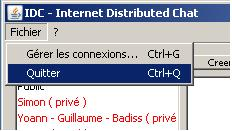
\includegraphics{screenIHMmenu.jpg}
\end{center}
\section{Description technique}
\subsection{Broadcast}

La fonction recherche disponible lorsqu'on veut gérer ses connexions
fait une demande sur le réseau local par broadcast. Tous les noeuds du
LAN reçoivent donc cette demande et se manifestent en envoyant leurs
informations au client qui fait la demande.\\

\subsection{Communications}

Un noeud du réseau n'est connecté qu'à ses pairs directs, ceux qu'il a ajoutés après avoir lancé l'application. Il n'y a pas de communication directe entre tous les pairs du réseau. Les informations qui doivent transiter d'un bout à l'autre du réseau sont routées de pair en pair. Les pairs avec qui un client est connecté sont appelés pairs directs ou connexions directes. D'un point de vue réseau, un client échange des données uniquement avec ses pairs directs.
Connexion directe et noeud du réseau

\paragraph{}
Une connexion directe est une connexion entre deux noeuds du réseau. Un client du réseau possède une connexion directe ou plus. Généralement il en possède plus de 3 pour que le réseau soit bien équilibré et qu'un noeud n'ait pas qu'une seule route possible pour communiquer avec les autres noeuds. Pour que deux noeuds A et B soient en connexion directe, il faut que :

\begin{itemize}
\item{A connaisse l'adresse ip et le port d'écoute de B}
\item{B connaisse l'adresse ip et le port d'écoute de A}
\end{itemize}

\subsection{Sur le réseau}

Un noeud A du réseau est défini sur le réseau par :

\begin{itemize}
\item{une chaine de caractère précisée par l'utilisateur (pour plus de convivialité). Cela peut être un nom ou un nickname.}
\item{un id. Cet id est une signature SHA de sa clef publique. La clef publique d'un noeud A est une clef de type RSA et sera unique sur le réseau. Seul A possedera la clef privée associée. C'est cette paire de clefs qui permettra de lancer des communication chiffrée entre deux pairs ou plus.}
\end{itemize}
\subsection{Exemple de communication chiffrée}

La mise en place d'une communication chiffrée entre deux clients A et B se déroulera de cette manière :
\begin{enumerate}
\item{A demande la clef publique de B grace à l'id de B.}
\item{B envoie sa clef publique et demande celle de A.}
\item{A réceptionne la clef publique et confirme l'identité de B grâce au calcul de la signature de la clef reçue qui doit correspondre à l'id de B.}
\item{A connait maintenant la clef publique de B et l'utilise pour chiffrer ses communications. Il envoie sa clef publique à B \textbf{(communication~chiffrée~RSA)}}
\item{B reçoit la clef de A. \textbf{(communication~chiffrée~RSA)}}
\item{B réceptionne la clef publique et confirme l'identité de A grâce au calcul de la signature de la clef reçue qui doit correspondre à l'id de A. \textbf{(communication~chiffrée~RSA)}}
\item{A propose une clef de session AES à B pour cette communication \textbf{(communication~chiffrée~RSA)}}
\item{B accepte la clef et le fait savoir à A \textbf{(communication~chiffrée~RSA)}}
\item{A et B s'envoient des données \textbf{(communication~chiffrée~AES)}}
\end{enumerate}

Cette communication n'est pas à l'abri de l'attaque "man in the
middle". C'est pour cette raison que l'utilisateur de l'application a
la possibilité d'afficher l'ensemble des clefs publiques qu'il a pu
récupérer sur le réseau. Il peut ainsi demander à la personne
concernée, en dehors de l'application si les clefs publiques qu'ils
possèdent correspondent bien.

\subsection{Routage}

Des algorithmes de routage tels que l'\textit{adaptive routing} ou le \textit{deflecting routing} seront probablement utilisés. L'algorithme de Dijkstra et de la vague serviront également.



\end{document}









